% =====================================================================
\lecture{4}{עדויות לחומר אפל: ויריאל, קריסה כדורית, עקומות סיבוב, \en{NFW} ו-\en{MOND}}{מפגש 2, שעה. \ (10' ויריאל, 15' קריסה כדורית, 20' עקומות סיבוב ופרופילים, 10' התאמה, 5' \en{MOND}, תרגילים)}
% =====================================================================

\begin{goalbox}
\textbf{מטרות.} (1) להעריך מסה ממהירויות: משפט הוויריאל. (2) לגזור את מודל הקריסה הכדורית ($\delta_c$, $18\pi^2$, $r_{\rm vir}$) ולהשתמש בו כעדות לחומר אפל (טיעון התזמון). (3) לקרוא עקומת סיבוב ולהסיק ממנה פרופיל צפיפות. (4) להכיר את פרופיל \en{NFW} ולהתאים אותו לנתונים (אותה מכונה של הרצאה 2). (5) לדעת מה \en{MOND} מסביר ומה לא.
\end{goalbox}

\subsection{משפט הוויריאל: צבירי גלקסיות}
למערכת כבולה במצב יציב, ממוצע בזמן של $\frac{d^2I}{dt^2}=0$ ($I=\sum m r^2$):
\begin{equation}
2K+W=0 .
\end{equation}
לכדור אחיד: $W=-\frac35\frac{GM^2}{R}$; ומהירות נמדדת רק לאורך קו הראייה, $K=\frac12M\langle v^2\rangle=\frac32M\sigma_{\rm los}^2$. לכן
\begin{equation}
\boxed{\;M\simeq\frac{5\,\sigma_{\rm los}^2R}{G}\;}
\end{equation}
\textbf{\en{Zwicky} (1933), צביר \en{Coma}:} $\sigma\approx1000\,\kms$, $R\approx1.5\,\Mpc$ נותנים $M\sim2\times10^{15}\Msun$ ויחס מסה-אור $M/L\sim300$ (בשמש: 1, בכוכבים: $\sim3$). היום: גז חם בקרני \en{X} ועדשות כבידה נותנים אותה תמונה. בריונים (בעיקר גז) הם $\sim15\%$ מהמסה, כמו $\Omega_b/\Omega_m$ הקוסמי.

\subsection{קריסה כדורית: איך נוצרת הילה כבולה}\label{sec:sc}
\en{Zwicky} הניח שהצביר בשיווי משקל ויריאלי. מודל הקריסה הכדורית (\en{Gunn \& Gott 1972}) מסביר למה, באיזו צפיפות, ובאיזה רדיוס. הוא גם נותן שני מבחנים לחומר אפל שאינם תלויים בשיווי משקל: מסת החבורה המקומית מהדינמיקה שלה בלבד, וגודל ההילה סביב גלקסיה, שאותו בודקות עקומות הסיבוב (סעיף הבא).

\textbf{משוואת הקליפה.} כדור שצפיפותו מעט גבוהה מהרקע. לפי משפט \en{Birkhoff}, קליפה ברדיוס $R(t)$ מרגישה רק את המסה $M$ שבתוכה (כל עוד הקליפות אינן חוצות זו את זו):
\begin{equation}
\ddot R=-\frac{GM}{R^2}+\frac{\Lambda}{3}R,\qquad
\frac12\dot R^2-\frac{GM}{R}-\frac{\Lambda}{6}R^2=E .
\label{eq:sc-eom}
\end{equation}
הילות נוצרות בעיקר בעידן החומר, ולכן נתחיל ב-$\Lambda=0$ ורקע \en{EdS}. עם $E<0$ הקליפה קשורה: זהו יקום פרידמן קטן עם $k=+1$ (הרצאה 1).

\textbf{הפתרון (ציקלואידה).}
\begin{equation}
\boxed{\;R=A(1-\cos\theta),\qquad t=B(\theta-\sin\theta),\qquad A^3=GMB^2\;}
\label{eq:sc-cycloid}
\end{equation}
בדיקה: $\dot R=\frac{dR/d\theta}{dt/d\theta}=\frac{A}{B}\frac{\sin\theta}{1-\cos\theta}$. עם $\sin^2\theta=(1-\cos\theta)(1+\cos\theta)$ ו-$GM=A^3/B^2$:
\begin{equation}
E=\frac{A^2}{B^2}\Big[\frac{1+\cos\theta}{2(1-\cos\theta)}-\frac{1}{1-\cos\theta}\Big]=-\frac{A^2}{2B^2},
\end{equation}
קבוע ושלילי, כנדרש.
\begin{center}\small
\begin{tabular}{@{}cccl@{}}
\toprule
$\theta$ & $R$ & $t$ & משמעות \\ \midrule
$0$ & $0$ & $0$ & ההפרעה מתחילה עם הרקע \\
$\pi$ & $R_{\rm ta}=2A$ & $t_{\rm ta}=\pi B$ & נקודת המפנה (\en{turnaround}), $\dot R=0$ \\
$2\pi$ & $0$ & $t_{\rm coll}=2t_{\rm ta}$ & קריסה (פורמלית) \\ \bottomrule
\end{tabular}
\end{center}

\textbf{הניגוד בצפיפות.} $\rho_{\rm sh}=3M/4\pi R^3$ ו-$\bar\rho=1/6\pi Gt^2$ (\en{EdS}). היחס, אחרי שימוש ב-$A^3=GMB^2$:
\begin{equation}
1+\delta(\theta)=\frac92\,\frac{(\theta-\sin\theta)^2}{(1-\cos\theta)^3}.
\label{eq:sc-dNL}
\end{equation}
התוצאה אינה תלויה ב-$M$: כל ההפרעות הכדוריות עוברות אותו מסלול, כל אחת בקצב שלה.

\textbf{הגבול הלינארי.} ל-$\theta\ll1$: $\theta-\sin\theta\simeq\frac{\theta^3}{6}(1-\frac{\theta^2}{20})$, $1-\cos\theta\simeq\frac{\theta^2}{2}(1-\frac{\theta^2}{12})$, ולכן $\delta\simeq\frac{3}{20}\theta^2$. עם $t\simeq B\theta^3/6$:
\begin{equation}
\delta_L(t)=\frac{3}{20}\Big(\frac{6t}{B}\Big)^{2/3}\propto a ,
\end{equation}
המוד הגדל של הרצאה 3. $\delta_L$ הוא מה שהתורה הלינארית \emph{הייתה} נותנת; את השדה הלינארי קל לחשב, ולכן הוא משמש כשעון. בשתי נקודות:
\begin{center}\small
\begin{tabular}{@{}lcc@{}}
\toprule
 & $\delta$ אמיתי & $\delta_L$ \\ \midrule
מפנה, $\theta=\pi$ & $\frac{9\pi^2}{16}-1=4.55$ & $\frac{3}{20}(6\pi)^{2/3}=1.06$ \\
קריסה, $\theta=2\pi$ & $\infty$ & $\boxed{\delta_c=\frac{3}{20}(12\pi)^{2/3}=1.686}$ \\ \bottomrule
\end{tabular}
\end{center}
הילה נוצרת היכן שהשדה הלינארי, מוחלק בסולם $R(M)$, חוצה את $\delta_c$. זה הבסיס של \en{Press--Schechter} ופונקציות המסה של הילות.

\textbf{ויריאליזציה: $18\pi^2$.} קריסה לנקודה היא תוצר של סימטריה מושלמת. בפועל תנועה רדיאלית הופכת לתנועה אקראית והמערכת מתייצבת. משפט הוויריאל $2K+W=0$ נותן $E=W/2$. במפנה $K=0$, ולכן $E=W_{\rm ta}$. מאחר ש-$W\propto-1/R$:
\begin{equation}
\frac{W_{\rm vir}}{2}=W_{\rm ta}\ \Longrightarrow\ \boxed{R_{\rm vir}=\tfrac12R_{\rm ta}} .
\end{equation}
המקדם ש-$W$ תלוי בו (פרופיל הצפיפות) מתבטל. הניגוד הסופי, ב-$t_{\rm coll}=2t_{\rm ta}$:
\begin{equation}
\Delta_{\rm vir}\equiv\frac{\rho_{\rm vir}}{\bar\rho(t_{\rm coll})}
=\underbrace{\frac{9\pi^2}{16}}_{\rm turnaround}\times\underbrace{2^3}_{R\to R/2}\times\underbrace{2^2}_{\bar\rho\propto t^{-2}}=18\pi^2\approx178 .
\end{equation}
מכאן הגדרת ההילה: המסה בתוך $r_{\rm vir}$, שבו הצפיפות הממוצעת היא $\Delta$ פעמים צפיפות הייחוס,
\begin{equation}
M_{\rm vir}=\frac{4\pi}{3}\Delta\,\rho_{\rm ref}\,r_{\rm vir}^3,\qquad V_{\rm vir}^2=\frac{GM_{\rm vir}}{r_{\rm vir}} .
\label{eq:sc-rvir}
\end{equation}

\textbf{עם $\Lambda$.} שלושה שינויים:
\begin{itemize}
\item $\delta_c$ כמעט לא משתנה: $\approx1.68$ ב-$\LCDM$ (תלות חלשה ב-$\Omega_m$).
\item $\Delta$ משתנה. התאמה נומרית ביחס לצפיפות הקריטית (\en{Bryan \& Norman 1998}): $\Delta_c=18\pi^2+82x-39x^2$, $x=\Omega_m(z)-1$. היום $\Delta_c\approx103$, כלומר $\approx330\bar\rho_m$. המוסכמה $M_{200}$ ($200\rho_c$) היא עיגול של אותו רעיון.
\item משפט הוויריאל מקבל איבר של $\Lambda$. לכדור אחיד $W_\Lambda=-\frac{\Lambda}{10}MR^2$, ומ-$2K=-W_G+2W_\Lambda$ (לאיבר $\propto R^n$, $2K=nW$) מתקבל $2K+W_G=2W_\Lambda$ (\en{Lahav et al.\ 1991}; להכללה לאנרגיה אפלה דינמית: \en{Naderi, Malekjani \& Pace 2015}). שימור אנרגיה בין המפנה לוויריאל נותן, עם $y=R_{\rm vir}/R_{\rm ta}$ ו-$Q=\rho_\Lambda/\rho_{\rm ta}$:
\begin{equation}
4Qy^3-2(1+Q)y+1=0,\qquad y\simeq\tfrac12-\tfrac{Q}{4}.
\end{equation}
$\Lambda$ דוחה, ולכן ההילה קורסת לרדיוס קטן יותר. ומ-\eqref{eq:sc-eom}: קליפה נעצרת רק אם $\ddot R<0$ במפנה, כלומר $R_{\rm ta}<(3GM/\Lambda)^{1/3}$, רדיוס מפנה מקסימלי ($1.1\,\Mpc$ ל-$10^{12}\Msun$, $11\,\Mpc$ ל-$10^{15}\Msun$; \en{Pavlidou \& Tomaras 2014}).
\end{itemize}

\begin{keybox}
\textbf{למה זו עדות לחומר אפל.}
\begin{enumerate}
\item \textbf{טיעון התזמון} (\en{Kahn \& Woltjer 1959}). שביל החלב ו-\en{M31} נמצאים ב-$r\approx0.78\,\Mpc$ ומתקרבים ב-$v_r\approx-110\,\kms$. אם נפרדו במפץ ונעים במסלול רדיאלי, הם על הציקלואידה \eqref{eq:sc-cycloid} עם $t=t_0$:
\begin{equation}
\frac{v\,t_0}{r}=\frac{\sin\theta\,(\theta-\sin\theta)}{(1-\cos\theta)^2}=-1.99
\ \Rightarrow\ \theta=4.20,\quad M=\frac{A^3}{GB^2}\approx4\times10^{12}\Msun
\end{equation}
(תרגיל 4.4). עם $\Lambda$ וכיול על סימולציות: $\sim5\times10^{12}\Msun$ (\en{Li \& White 2008}). הכוכבים והגז בשתי הגלקסיות: $\sim2\times10^{11}\Msun$. חסר פקטור $\sim20$. החישוב משתמש רק בכבידה ובגיל היקום, בלי הנחה על שיווי משקל.
\item \textbf{גודל ההילה.} הילה של $10^{12}\Msun$ היום: מ-\eqref{eq:sc-rvir} עם $\Delta_c=103$, $r_{\rm vir}\approx260\,\kpc$ ו-$V_{\rm vir}\approx130\,\kms$. הדיסקה הכוכבית נגמרת ב-$\sim15$--$20\,\kpc$. החיזוי: מסה שמשתרעת פי $\sim10$ מעבר לאור, ומהירויות סיבוב של $\sim100$--$200\,\kms$ הרחק מהדיסקה (הריכוז, סעיף~\ref{sec:nfw}, מעלה את $v_c$ בפנים). זה בדיוק מה שעקומות הסיבוב בודקות.
\item \textbf{מתי.} הילה נוצרת כש-$\delta_L$ מגיע ל-$1.686$. בריונים לבדם מגיעים היום ל-$\delta_L\sim10^{-2}$ (הרצאה 3), כלומר לא הייתה נוצרת אף הילה. עם \en{CDM}, הילות בגודל גלקסיה קורסות ב-$z\sim1$--$3$.
\end{enumerate}
\end{keybox}

\subsection{עקומות סיבוב}
למסלול מעגלי בפוטנציאל כדורי:
\begin{equation}
v_c^2(r)=\frac{GM(<r)}{r}.
\end{equation}
\begin{itemize}
\item מחוץ לרוב המסה הנראית: $v_c\propto r^{-1/2}$ (קפלר).
\item נצפה (\en{Rubin}, קווי \en{HI} באורך 21 ס"מ, 1970--80): $v_c\approx$ קבוע עד רדיוסים גדולים בהרבה מהדיסקה.
\item $v_c=$ קבוע $\Rightarrow M(<r)\propto r\Rightarrow\rho\propto r^{-2}$: \textbf{הילה איזותרמית}.
\end{itemize}
המהירות הכוללת היא סכום ריבועים של הרכיבים (פואסון לינארי):
\begin{equation}
v_c^2=\Upsilon_\star v_\star^2+v_{\rm gas}^2+v_{\rm DM}^2,
\end{equation}
עם $\Upsilon_\star$ יחס מסה-אור של הכוכבים. לדיסקה אקספוננציאלית ($\Sigma\propto e^{-R/R_d}$) $v_\star$ מגיעה לשיא ב-$2.2R_d$ ויורדת.

\subsection{פרופילי הילה}\label{sec:nfw}
\begin{keybox}
\textbf{\en{NFW}} (\en{Navarro, Frenk \& White 1997}) --- פרופיל אוניברסלי של הילות בסימולציות \en{CDM}:
\begin{equation}
\rho(r)=\frac{\rho_s}{(r/r_s)(1+r/r_s)^2},\qquad
M(<r)=4\pi\rho_sr_s^3\Big[\ln(1+x)-\frac{x}{1+x}\Big],\ \ x=r/r_s .
\end{equation}
$\rho\propto r^{-1}$ במרכז (\textbf{קאספ}) ו-$r^{-3}$ בחוץ. המסה מתבדרת לוגריתמית, ולכן מגדירים $M_{200}$: המסה בתוך $r_{200}$ שבו הצפיפות הממוצעת $=200\rho_c$. פרמטר הריכוז $c=r_{200}/r_s\sim5$--$15$, ויורד לאט עם המסה. $v_c$ מקסימלית ב-$r=2.163\,r_s$.
\end{keybox}
\textbf{ליבות מול קאספים.} בגלקסיות ננס רבות הנתונים מעדיפים ליבה, $\rho\to$ קבוע: איזותרמית-מדומה $\rho_0/[1+(r/r_c)^2]$ או \en{Burkert} $\rho_0r_0^3/[(r+r_0)(r^2+r_0^2)]$. הסבר אפשרי: משוב מסופרנובות שמזיז גז ושוטח את המרכז. או חומר אפל שאינו קר לגמרי (\en{SIDM}, \en{fuzzy DM}).

\subsection{התאמת פרופיל לעקומת סיבוב}
אותה מכונה של הרצאה 2:
\begin{enumerate}
\item נתונים: $(r_i,v_i,\sigma_i)$; רכיבים בריוניים $v_\star(r),v_{\rm gas}(r)$ מפוטומטריה ומ-\en{HI}.
\item מודל: $v^2=\Upsilon_\star v_\star^2+v_{\rm gas}^2+v_{\rm NFW}^2(r;M_{200},c)$.
\item $\chi^2=\sum_i(v_i-v(r_i))^2/\sigma_i^2$; מוקדמות: $\Upsilon_\star$ מאוכלוסיות כוכבים, יחס $c(M)$ מסימולציות.
\item \en{MCMC} על $(\log M_{200},c,\Upsilon_\star)$ ו-\en{corner}.
\end{enumerate}
\textbf{ניוון דיסקה-הילה:} דיסקה כבדה יותר ($\Upsilon_\star$ גדול) מפוצה בהילה עם ריכוז נמוך. זו אותה בננה שראינו ב-$(\Omega_m,w)$. ההנחה "דיסקה מקסימלית" היא הגבול העליון של הניוון.

\begin{figure}[htbp]\centering
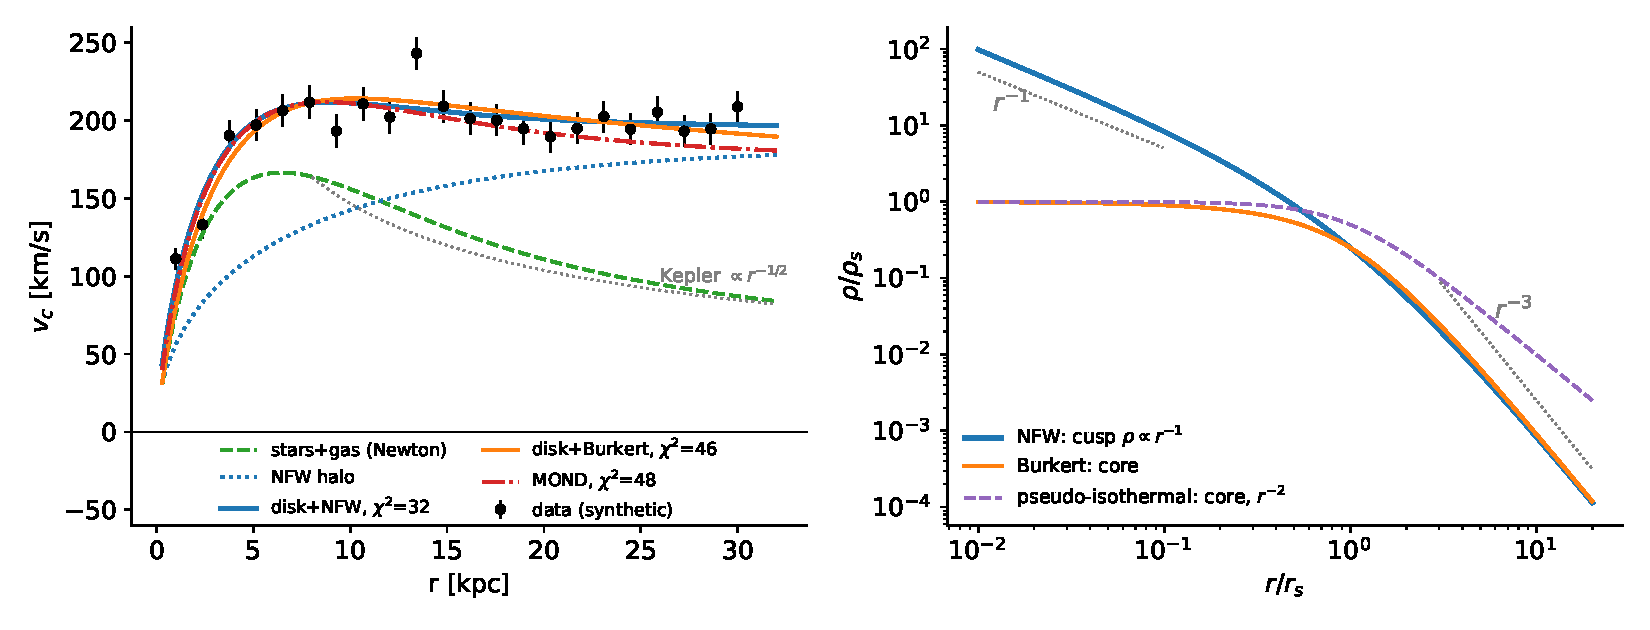
\includegraphics[width=\textwidth]{figs/fig_rotcurve_nfw.pdf}
\caption{\small שמאל: עקומת סיבוב סינתטית (נוצרה מ-\en{NFW}), מותאמת בדיסקה+\en{NFW}, דיסקה+\en{Burkert}, ו-\en{MOND} ללא חומר אפל. הכוכבים לבדם (ירוק) יורדים כמו קפלר; הנתונים לא. ימין: צורת הפרופילים --- קאספ מול ליבה. הסקריפט: \en{scripts/make\_new\_figs.py}.}
\end{figure}

\subsection{עדויות נוספות (בקצרה)}
עדשות כבידה חזקות וחלשות ממפות מסה ישירות; \en{Bullet Cluster}: מרכז המסה (עדשות) נפרד מהגז החם (קרני \en{X}) אחרי התנגשות; ה-\en{CMB}: יחס גובה הפסגות האי-זוגיות לזוגיות דורש $\Omega_ch^2\approx0.12$ (הרצאה 5); וצמיחת מבנה (הרצאה 3).

\subsection{\en{MOND} --- בקצרה}
\en{Milgrom} (1983): לא חומר חסר אלא דינמיקה שונה בתאוצות נמוכות.
\begin{equation}
\mu\!\Big(\frac{g}{a_0}\Big)\,g=g_N,\qquad a_0\approx1.2\times10^{-10}\,\mathrm{m\,s^{-2}},\qquad \mu(x)\to\begin{cases}1&x\gg1\\x&x\ll1\end{cases}
\end{equation}
בגבול העמוק $g=\sqrt{g_Na_0}$, ומ-$v^2/r=\sqrt{GMa_0}/r$:
\begin{equation}
v_{\rm flat}^4=GM_ba_0 \qquad(\text{\en{baryonic Tully--Fisher}}).
\end{equation}
\begin{center}\small
\begin{tabular}{@{}p{7cm}p{7cm}@{}}
\toprule
\textbf{הצלחות} & \textbf{קשיים} \\ \midrule
עקומות סיבוב של גלקסיות עם פרמטר אחד ($a_0$) & צבירים: עדיין חסר פקטור $\sim2$ במסה \\
יחס \en{Tully--Fisher} הבריוני, כולל השיפוע 4 & \en{Bullet Cluster}: המסה לא עוקבת אחרי הבריונים \\
הקשר ההדוק $g_{\rm obs}(g_{\rm bar})$ (\en{RAR}) & ה-\en{CMB} וספקטרום ההספק: ללא רכיב לא-בריוני --- פסגה שלישית נמוכה מדי \\
& אין תיאוריה יחסותית פשוטה ומקובלת (\en{TeVeS} נפסלה עם \en{GW170817}) \\ \bottomrule
\end{tabular}
\end{center}
המסקנה המקובלת: \en{MOND} הוא תיאור מוצלח של \emph{גלקסיות}, וכל מודל חומר אפל חייב לשחזר את ה-\en{RAR}; בסולמות קוסמולוגיים \en{CDM} עדיף בבירור.

% ---------------------------------------------------------------------
\subsection*{תרגילים}
\begin{exercise}{\en{Zwicky} ו-\en{Coma}}
(א) גזרו $M=5\sigma_{\rm los}^2R/G$ ממשפט הוויריאל לכדור אחיד. (ב) עם $\sigma_{\rm los}=1000\,\kms$, $R=1.5\,\Mpc$ ו-$L\approx5\times10^{12}L_\odot$ חשבו $M$ ו-$M/L$. (ג) זמן החצייה $R/\sigma$ --- האם הוא קצר מגיל היקום? למה זה חשוב לשימוש בוויריאל?
\end{exercise}
\begin{solbox}
\textbf{פתרון.}\ (א) $2K+W=0$, $K=\tfrac32M\sigma^2$, $W=-\tfrac35GM^2/R\Rightarrow M=5\sigma^2R/G$.\\
(ב) $M=5(10^6)^2(4.6\times10^{22})/6.67\times10^{-11}=3.5\times10^{45}\,\mathrm{kg}=1.7\times10^{15}\Msun$. $M/L\approx350$.\\
(ג) $R/\sigma=1.5\,\Gyr\ll t_0$: הצביר עבר כמה זמני חצייה, ולכן סביר שהוא קרוב לשיווי משקל ויריאלי.
\end{solbox}

\begin{exercise}{פרופיל \en{NFW}}
(א) גזרו את $M(<r)$ מ-$\rho_{\rm NFW}$. (ב) מצאו את האסימפטוטות של $v_c(r)$ ב-$r\ll r_s$ וב-$r\gg r_s$. (ג) הראו ש-$v_c$ מקסימלית כאשר $\ln(1+x)=\frac{x(2x+1)}{(1+x)^2}$, ופתרו נומרית ($x\approx2.16$). (ד) לגלקסיה עם $v_{\max}=200\,\kms$ ב-$r_{\max}=40\,\kpc$, מצאו $r_s$ ו-$\rho_s$.
\end{exercise}
\begin{solbox}
\textbf{פתרון.}\ (א) $M=4\pi\rho_sr_s^3\int_0^x\frac{x'\,dx'}{(1+x')^2}=4\pi\rho_sr_s^3[\ln(1+x)-\frac{x}{1+x}]$.\\
(ב) $x\ll1$: $M\approx2\pi\rho_sr_s^3x^2$, $v\propto r^{1/2}$. $x\gg1$: $M\propto\ln x$, $v^2\propto\ln r/r$ (יורד לאט).\\
(ג) $\frac{d}{dx}[m(x)/x]=0\Rightarrow xm'=m$, $m'=x/(1+x)^2$. מכאן $\ln(1+x)=\frac{x}{1+x}+\frac{x^2}{(1+x)^2}=\frac{x(2x+1)}{(1+x)^2}$; $x=2.163$, $m(x)/x=0.2162$.\\
(ד) $r_s=40/2.163=18.5\,\kpc$. $v_{\max}^2=4\pi G\rho_sr_s^2\times0.2162\Rightarrow\rho_s=1.0\times10^7\Msun\,\kpc^{-3}$.
\end{solbox}

\begin{exercise}{\en{MOND} בגלקסיה אחת}
גלקסיה עם $M_b=6\times10^{10}\Msun$. (א) באיזה רדיוס $r_M$ התאוצה הניוטונית משתווה ל-$a_0$? (ב) מה $v_{\rm flat}$ שחוזה \en{MOND}? (ג) ב-$r=30\,\kpc$ (נקודה מסה): חשבו $v$ ניוטוני ו-$v$ של \en{MOND} עם $\mu(x)=x/(1+x)$. (ד) גלקסיה עם מסה בריונית גדולה פי 16: פי כמה $v_{\rm flat}$?
\end{exercise}
\begin{solbox}
\textbf{פתרון.}\ (א) $r_M=\sqrt{GM_b/a_0}=8.3\,\kpc$.\\
(ב) $v_{\rm flat}=(GM_ba_0)^{1/4}=176\,\kms$.\\
(ג) $v_N=\sqrt{GM/r}=93\,\kms$. $g=\tfrac12g_N+\sqrt{g_N^2/4+g_Na_0}$ עם $g_N=9.3\times10^{-12}\,\mathrm{m\,s^{-2}}$: $g=3.8\times10^{-11}$, $v=188\,\kms$ (ושואף ל-176 ברדיוס גדול). כמו שחומר אפל היה נותן.\\
(ד) $16^{1/4}=2$. ב-\en{CDM} היחס הזה אינו נובע אוטומטית; הוא דורש שהבריונים יעקבו אחרי ההילה.
\end{solbox}

\begin{exercise}{טיעון התזמון של החבורה המקומית}
(א) מהציקלואידה \eqref{eq:sc-cycloid} הראו ש-$\frac{vt}{r}=\frac{\sin\theta(\theta-\sin\theta)}{(1-\cos\theta)^2}$. (ב) עם $r=0.78\,\Mpc$, $v=-110\,\kms$ ו-$t_0=13.8\,\Gyr$, פתרו נומרית ל-$\theta$ (רמז: הזוג כבר אחרי המפנה, $\pi<\theta<2\pi$) ומצאו $A$, $B$ ו-$M$. (ג) מה היה המרחק המקסימלי ומתי? (ד) השוו למסה הבריונית $\sim2\times10^{11}\Msun$. (ה) איך ישתנה $M$ אם $|v|$ גדל ב-10\%?
\end{exercise}
\begin{solbox}
\textbf{פתרון.}\ (א) $v=\dot R=\frac AB\frac{\sin\theta}{1-\cos\theta}$, $t/r=\frac{B(\theta-\sin\theta)}{A(1-\cos\theta)}$; המכפלה נותנת את הביטוי.\\
(ב) ביחידות $1\,\Mpc/\kms=977.8\,\Gyr$: $t_0=0.01411\,\Mpc/\kms$, ולכן $vt_0/r=-110\times0.01411/0.78=-1.99$. פתרון: $\theta=4.20$. $A=r/(1-\cos\theta)=0.523\,\Mpc$, $B=t_0/(\theta-\sin\theta)=2.72\,\Gyr$. $M=A^3/GB^2=4.3\times10^{12}\Msun$ (עם $G=4.30\times10^{-9}\,\Mpc\,(\kms)^2/\Msun$).\\
(ג) $R_{\max}=2A=1.05\,\Mpc$ ב-$t_{\rm ta}=\pi B=8.5\,\Gyr$, לפני כ-5 מיליארד שנה.\\
(ד) $M/M_b\approx20$: רוב המסה של החבורה המקומית אינה בכוכבים ובגז.\\
(ה) $|v|=121\,\kms$: $M\approx4.8\times10^{12}\Msun$, עלייה של $\sim11\%$. התוצאה חסינה יחסית לשגיאות במהירות.
\end{solbox}
